\subsection{柯西积分定理}
\label{subsec:cauchy_theorem}
柯西积分定理(简称柯西定理)说的是,如果$f(z)$是解析函数,$f'(z)$在闭合路径$C$%构成的单连通
区域内任一点连续,有
\begin{equation}
    \oint_C f(z) dz = 0.
\end{equation}
所有的闭合回路的积分我们用$\oint$来表示.证明会用到格林公式和柯西-黎曼条件,具体参考其他书目,其中
格林公式为
\begin{equation}
    \oint_\ell P dx + Q dy = \iint_S \left( \frac{\partial Q}{\partial x} - \frac{\partial P}{\partial y} dx dy \right)
\end{equation}
对于某些区域有奇点的情况,我们可以取一绕过奇点的闭合路径,如图\ref{fig:complexregion}所示的情况.柯西定理重要的应用在于将沿某一路径积分转化为
另一个或多个路径积分的求和.通常这样来规定正方向,当观察者沿着该方向前进时,区域总是在观察者的左侧.
\begin{figure}
    \centering
    

\tikzset{every picture/.style={line width=0.75pt}} %set default line width to 0.75pt        

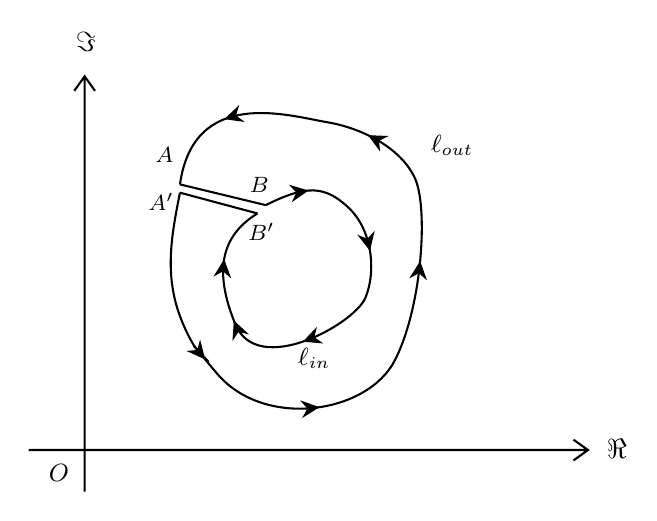
\begin{tikzpicture}[x=0.75pt,y=0.75pt,yscale=-1,xscale=1]
%uncomment if require: \path (0,300); %set diagram left start at 0, and has height of 300

%Shape: Axis 2D [id:dp04611299520330148] 
\draw  (107,219.06) -- (376.47,219.06)(133.95,39) -- (133.95,239.07) (369.47,214.06) -- (376.47,219.06) -- (369.47,224.06) (128.95,46) -- (133.95,39) -- (138.95,46)  ;
%Curve Lines [id:da4408212979573587] 
\draw    (179.87,91.07) .. controls (186.53,43.73) and (232.62,58.07) .. (250.53,61.07) .. controls (268.45,64.07) and (286.87,74.07) .. (293.2,88.4) .. controls (299.53,102.73) and (296.53,150.4) .. (283.33,175.97) .. controls (270.13,201.54) and (220.5,209.23) .. (197.65,182.12) .. controls (174.81,155.01) and (194.63,178.2) .. (193.33,175.97) ;
\draw [shift={(201.24,59.65)}, rotate = 342.17] [fill={rgb, 255:red, 0; green, 0; blue, 0 }  ][line width=0.08]  [draw opacity=0] (8.93,-4.29) -- (0,0) -- (8.93,4.29) -- (5.93,0) -- cycle    ;
\draw [shift={(270.48,67.37)}, rotate = 27.92] [fill={rgb, 255:red, 0; green, 0; blue, 0 }  ][line width=0.08]  [draw opacity=0] (8.93,-4.29) -- (0,0) -- (8.93,4.29) -- (5.93,0) -- cycle    ;
\draw [shift={(295.59,127.97)}, rotate = 96.21] [fill={rgb, 255:red, 0; green, 0; blue, 0 }  ][line width=0.08]  [draw opacity=0] (8.93,-4.29) -- (0,0) -- (8.93,4.29) -- (5.93,0) -- cycle    ;
\draw [shift={(247.14,198.42)}, rotate = 173.71] [fill={rgb, 255:red, 0; green, 0; blue, 0 }  ][line width=0.08]  [draw opacity=0] (8.93,-4.29) -- (0,0) -- (8.93,4.29) -- (5.93,0) -- cycle    ;
\draw [shift={(192.02,175.42)}, rotate = 230.07] [fill={rgb, 255:red, 0; green, 0; blue, 0 }  ][line width=0.08]  [draw opacity=0] (8.93,-4.29) -- (0,0) -- (8.93,4.29) -- (5.93,0) -- cycle    ;
%Straight Lines [id:da2752936846063838] 
\draw    (179.87,91.07) -- (221.2,101.07) ;
%Curve Lines [id:da2227786948358368] 
\draw    (221.2,101.07) .. controls (241.2,91.07) and (249.87,91.73) .. (261.2,102.4) .. controls (272.53,113.07) and (274.53,133.07) .. (269.2,145.73) .. controls (263.87,158.4) and (217.2,184.4) .. (206.53,158.4) .. controls (206.05,157.22) and (205.59,156.05) .. (205.17,154.91) .. controls (196.26,130.89) and (200.66,115.25) .. (217.2,105.07) ;
\draw [shift={(241.83,94.03)}, rotate = 170.78] [fill={rgb, 255:red, 0; green, 0; blue, 0 }  ][line width=0.08]  [draw opacity=0] (8.93,-4.29) -- (0,0) -- (8.93,4.29) -- (5.93,0) -- cycle    ;
\draw [shift={(271.41,123.08)}, rotate = 257.51] [fill={rgb, 255:red, 0; green, 0; blue, 0 }  ][line width=0.08]  [draw opacity=0] (8.93,-4.29) -- (0,0) -- (8.93,4.29) -- (5.93,0) -- cycle    ;
\draw [shift={(239.05,166.85)}, rotate = 339.24] [fill={rgb, 255:red, 0; green, 0; blue, 0 }  ][line width=0.08]  [draw opacity=0] (8.93,-4.29) -- (0,0) -- (8.93,4.29) -- (5.93,0) -- cycle    ;
\draw [shift={(205.83,156.66)}, rotate = 68.16] [fill={rgb, 255:red, 0; green, 0; blue, 0 }  ][line width=0.08]  [draw opacity=0] (8.93,-4.29) -- (0,0) -- (8.93,4.29) -- (5.93,0) -- cycle    ;
\draw [shift={(201.16,127.05)}, rotate = 95.63] [fill={rgb, 255:red, 0; green, 0; blue, 0 }  ][line width=0.08]  [draw opacity=0] (8.93,-4.29) -- (0,0) -- (8.93,4.29) -- (5.93,0) -- cycle    ;
%Straight Lines [id:da5896769090029934] 
\draw    (179.87,95.07) -- (217.2,105.07) ;
%Curve Lines [id:da07734592378285976] 
\draw    (187.2,169.73) .. controls (171.07,142.83) and (174.53,121.73) .. (179.87,95.07) ;

% Text Node
\draw (115.17,224.57) node [anchor=north west][inner sep=0.75pt]  [font=\small]  {$O$};
% Text Node
\draw (299.33,66.07) node [anchor=north west][inner sep=0.75pt]  [font=\small]  {$\ell _{out}$};
% Text Node
\draw (166.67,71.73) node [anchor=north west][inner sep=0.75pt]  [font=\footnotesize]  {$A$};
% Text Node
\draw (211.33,108.4) node [anchor=north west][inner sep=0.75pt]  [font=\footnotesize]  {$B'$};
% Text Node
\draw (212,86.4) node [anchor=north west][inner sep=0.75pt]  [font=\footnotesize]  {$B$};
% Text Node
\draw (163.33,93.73) node [anchor=north west][inner sep=0.75pt]  [font=\footnotesize]  {$A'$};
% Text Node
\draw (235.33,168.73) node [anchor=north west][inner sep=0.75pt]  [font=\small]  {$\ell _{in}$};
% Text Node
\draw (128.17,16.07) node [anchor=north west][inner sep=0.75pt]    {$\Im $};
% Text Node
\draw (384,212.4) node [anchor=north west][inner sep=0.75pt]    {$\Re $};


\end{tikzpicture}

    \caption{复杂路径示意图.}
    \label{fig:complexregion}
\end{figure}
由于$\ell_{in}$和$\ell_{out}$与割线$AB,A'B'$组成了闭合回路,根据柯西定理,我们有
\[
    \left[ \oint _{\ell_{out}} + \int _{\ell_{AB}} + \oint _{\ell_{in}} + \int _{\ell_{B'A'}} \right] f(z) dz = 0 .
\]   
由于割线$AB$与$A'B'$可以无限接近,可以看出二者方向相反,这两项互相抵消.于是我们有
\[
    \left[ \oint _{\ell_{out}} + \oint _{\ell_{in}}  \right] f(z) dz = 0,
\]
即
\[
    \oint_{\ell_{out}} f(z) dz = - \oint _{\ell_{in}}f(z) dz .
\]
若用逆时针方向积分表示,并考虑多个内边界$\ell_{i}$,我们有
\begin{equation}
    \ointctrclockwise_{\ell_{out}} f(z) dz = \sum_{i=1}^{n} \ointctrclockwise_{\ell_{in}} f(z) dz .
\end{equation}
就是说,外边界逆时针方向积分等于所有内边界逆时针方向积分之和.只要积分起点和终点固定,当积分路径连续变形时(即不跳过奇点),函数的积分值不变.

下面给出一个重要的例题.
\begin{examplebox}{计算积分\[ I = \oint_\ell (z-\alpha)^n dz, \]其中$n$为整数.}
首先,有柯西定理易知,若回路$\ell$不包含$\alpha$,则被积函数在$\ell$所围区域上是解析的,故积分值为零.下面讨论$\ell$包围$\alpha$的情形.
如果$n\geq 0$,被积函数在$\ell$所围区域是解析的,积分为零.若$n<0$,则有一个奇点$\alpha$.取以$\alpha$为圆心半径为$R$的圆周$C$,$R$大小任意.
于是圆周上有$z-\alpha = Re^{\imath \theta}$.
\begin{equation}
\begin{aligned}
    I &= \oint_\ell (z-\alpha)^n dz\\
     &= \oint_c R^n e^{\imath n \theta} d (\alpha + R e^{\imath \theta})\\
     & =  \imath R^{n+1} \int_0^{2\pi} e^{\imath (n+1)\theta}  d\theta \\
     & = 0 \quad \textrm{if} \quad n\neq -1.
\end{aligned}
\end{equation}
当$n = -1$时, $I = 2\pi \imath$.其实,从原函数的角度来看,这个结果很容易理解.当$n\neq -1$,原函数为$(z-\alpha)^{n+1}/(n+1)$, 绕$\alpha$一周
原函数变化量为零.而当$n=-1$时,原函数时$\ln(z-\alpha)$, 绕一周变化量为$2\pi \imath$.因此我们得到了非常重要的表达式
\begin{equation}
    \begin{aligned}
        & \frac{1}{2 \pi \mathrm{i}} \oint_l \frac{\mathrm{d} z}{z-\alpha}= \begin{cases}0 & (l \text { 不包围 } \alpha), \\
        1 & (l \text { 包围 } \alpha) . \end{cases} \\
        & \frac{1}{2 \pi \mathrm{i}} \oint_l(z-\alpha)^n \mathrm{~d} z=0 \quad(n \neq-1) .
        \end{aligned}
\end{equation}
\end{examplebox}